\documentclass[table, 11pt]{article}
\usepackage[review]{acl}

% Standard package includes
\usepackage{booktabs}
\usepackage{bm}
\usepackage{tikz}
\usetikzlibrary{bayesnet,calc}
\usepackage{times}
\usepackage{latexsym}
\usepackage{amsmath}
\usepackage{amsthm}
\usepackage{makecell}
\usepackage{amssymb}
\usepackage{dsfont}
\usepackage{graphicx}
\usepackage{subcaption}
\usepackage{threeparttable}
\usepackage{algorithm}
\usepackage{algorithmic}
\usepackage{float}
\usepackage{amsfonts}
\usepackage{enumitem}
\renewcommand{\algorithmicrequire}{\textbf{Input:}}
\renewcommand{\algorithmicensure}{\textbf{Output:}}

\usepackage[T1]{fontenc}
\usepackage[utf8]{inputenc}
\usepackage{microtype}
\usepackage{inconsolata}
\usepackage{multirow}
\usepackage[normalem]{ulem}



\definecolor{lightgray}{gray}{0.80}
\definecolor{darkgreen}{rgb}{0.0, 0.5, 0.0}

\newtheorem{definition}{Definition}
\newtheorem{proposition}{Proposition}
\newtheorem{theorem}{Theorem}
\newtheorem{lemma}{Lemma}
\newtheorem{corollary}{Corollary}
\DeclareMathOperator{\Ncut}{Ncut}
\DeclareMathOperator{\vol}{vol}
\DeclareMathOperator{\cut}{cut}
\DeclareMathOperator{\supp}{supp}
\DeclareMathOperator{\tr}{tr}
\DeclareMathOperator{\sign}{sign}
\DeclareMathOperator{\layer}{layer}
\DeclareMathOperator*{\argmin}{arg\,min}
\DeclareMathOperator*{\argmax}{arg\,max}

\title{Automated Summarization of Attribution Graphs \\
as a Unified Optimization Problem}

\author{}

\begin{document}

\maketitle

\begin{abstract}
Mechanistic interpretability seeks to understand large language models
by identifying the causal pathways responsible for their behavior.
Circuit tracing methods produce attribution graphs encoding directed
influence among model components, but these graphs routinely contain
thousands of nodes and millions of edges, making manual inspection
impractical. Prior summarization pipelines combine pruning,
clustering, and DAG repair as a sequence of ad-hoc steps without an
overarching objective, leaving it unclear what is being optimized,
which approximations are being made, and where the algorithm has
slack. We formulate attribution-graph summarization as a single
constrained optimization problem over a pruned subgraph and a
supernode partition, with two terms corresponding to attribution
faithfulness and bidirectional concept coherence (with readability
balance handled implicitly by the cut's volume denominators), plus
hard constraints encoding DAG integrity, layer span, and a
complexity budget. The granularity hyperparameter $K$ is selected
externally via grid search under a graph-theoretic criterion (the
mean of supernode-graph quality measures). We then show that the
ASG pipeline---rank-percentile pruning, spectral clustering on a
layer-decayed bidirectional affinity, and DAG-feasibility
projection---is exactly a block-coordinate descent strategy on this
objective, with one principled relaxation or projection per block.
This framing exposes each hyperparameter as a Lagrange multiplier or
structural choice and locates the algorithm's optimality gaps.
\end{abstract}

\section{Introduction}\label{sec:intro}

The internal computations of large language models remain poorly
understood. Mechanistic interpretability has emerged as a key
approach for improving transparency, reliability, and controllability
by identifying the causal pathways underlying specific model
behaviors. Sparse autoencoders (SAEs) decompose activations into
interpretable features, and transcoders connect these features across
layers, enabling the construction of full \emph{attribution graphs}
encoding directed linear influence among features, attention heads,
embedding nodes, and logits.

The resulting graphs are typically too large to inspect by hand:
thousands of nodes, millions of edges. Summarization pipelines
therefore aim to produce a compact \emph{supernode graph} that
preserves the causal story while being small enough to read. A
representative such pipeline first \emph{prunes} the attribution
graph by keeping the most influence- and relevance-bearing nodes and
edges, then \emph{clusters} the surviving features into supernodes by
some affinity, then \emph{repairs} the induced supernode graph to be
a DAG. Each step is reasonable in isolation, but the overall
procedure is presented as a sequence of choices rather than as the
solution to a clearly stated problem. Several questions remain
unanswered in this presentation:

\begin{enumerate}[leftmargin=*,topsep=2pt,itemsep=2pt]
\item What single criterion is being optimized?
\item Which steps are exact and which are approximations?
\item What is the meaning of each hyperparameter
($\eta_V, \eta_E, \alpha, \lambda$, the mean operator $F_{\text{mean}}$,
$K$)?
\item Where in the pipeline is the largest improvement headroom?
\end{enumerate}

\paragraph{Our contribution.} We formulate attribution-graph
summarization as a single constrained optimization problem
$\mathcal{J}_K(V', E', \varphi)$ over the pruned subgraph $(V', E')$
and the supernode partition $\varphi$ at fixed granularity $K$, and
show that the standard summarization pipeline is exactly a
block-coordinate-descent strategy on $\mathcal{J}_K$.
The granularity $K$ is selected by an external grid search under a
graph-theoretic criterion---the mean of the supernode-graph quality
measures reported in evaluation. Concretely:

\begin{itemize}[leftmargin=*,topsep=2pt,itemsep=2pt]
\item We state criteria in words corresponding to the desiderata of
the summarization task (Section~\ref{sec:desiderata}), and translate
them into two objective terms plus three feasibility constraints
(Section~\ref{sec:objective}), with~(C3) handled implicitly by the
cut volumes.
\item We give the closed-form objective $\mathcal{J}_K$ with each
term tied to one criterion and each constraint tied to one
desideratum (Equation~\ref{eq:objective}).
\item We show the pipeline---rank-percentile cumulative-mass pruning,
spectral clustering on a layer-decayed bidirectional affinity, and
two-step DAG projection---is the block-coordinate descent strategy
where Block~1 is solved per-subproblem by greedy knapsack, Block~2
is solved by Shi--Malik spectral relaxation, and Block~3 is a
greedy feasibility projection (Section~\ref{sec:solution}).
\item We give the explicit $K$-selection criterion as a grid search
maximizing the mean over the supernode-graph quality columns
(Section~\ref{sec:k-selection}).
\end{itemize}

This framing makes precise what was previously implicit. Each
hyperparameter has a role: $\eta_V, \eta_E$ are derived from the
duals of the complexity budget, $\lambda$ is the dual of the
layer-span constraint, $\alpha$ is the log-pooling temperature in
the combined-evidence score, $F_{\text{mean}}$ is the strictness of
the ``both axes agree'' rule for bidirectional similarity, and $K$
is selected externally rather than optimized.

\section{Related Work}

\paragraph{Mechanistic interpretability and circuit tracing.}
A growing body of work seeks algorithmic explanations of transformer
behavior \cite{olah2020zoom, elhage2021mathematical}. Sparse
autoencoders \cite{cunningham2023sparse, bricken2023monosemanticity}
and cross-layer transcoders \cite{lindsey2024sparse} decompose
activations into interpretable features and connect them across
layers, enabling the construction of full attribution graphs
\cite{ameisen2024scaling}. Studies of indirect object identification
\cite{wang2022interpretability} and greater-than comparison
\cite{hanna2023does} have produced useful findings but rely on
hand-curated subgraphs. Frameworks for automating attribution
computation \cite{ameisen2024scaling} produce full attribution
graphs; the downstream summarization step has received less attention.

\paragraph{Graph summarization.}
Graph summarization broadly admits a taxonomy of grouping-,
attribute-, simplification-, and compression-based methods
\cite{liu2018graph}. Most work targets generic graphs or networks
with attribute side-information; the attribution-graph setting differs
in that nodes carry layer indices, edges carry signed continuous
weights, and the desideratum of DAG integrity is paramount. Spectral
clustering \cite{shi2000normalized, von2007tutorial} provides the
standard machinery for normalized-cut objectives and underlies the
clustering step we analyze. Modularity-based community detection
\cite{newman2006modularity, clauset2004finding} is the closest baseline
in the empirical evaluation. Higher-order Cheeger inequalities
\cite{lee2014multiway, louis2012many} give the approximation
guarantees for the spectral relaxation we analyze.

\paragraph{Pruning and attribution selection.}
The cumulative-mass thresholding rule we analyze is the same rule
used in prior circuit-tracing work to prune attribution graphs by
single-criterion mass coverage \cite{ameisen2024scaling}, applied
here to a combined influence-relevance ranking. The geometric-mean
combiner connects to log-linear pooling of independent rank
evidences \cite{genest1986combining}.

\paragraph{Position relative to prior summarization pipelines.}
Existing summarization steps in the circuit-tracing literature are
presented as algorithmic procedures rather than as solutions to a
stated optimization problem. We make the problem explicit and show
the procedure is a coordinate-descent strategy on it.


\section{Problem Formulation}\label{sec:setup}

We approach the problem in four movements. Section~\ref{sec:input}
fixes the input: a directed acyclic attribution graph together with
side data identifying its token and logit ends. Section~\ref{sec:output}
characterizes the output: a pruned subgraph together with a
supernode partition that groups surviving nodes into clusters.
Section~\ref{sec:desiderata} states three criteria a good summary
should satisfy---faithfulness, coherence, and readability---along
with the structural requirements (DAG integrity, layer locality,
budget) that any well-formed summary must respect.
Section~\ref{sec:operationalize} turns each criterion into a
measurable quantity defined on the input, and
Section~\ref{sec:objective} assembles those quantities into a
single constrained objective $\mathcal{J}_K$ that the rest of the
paper will solve.

\subsection{Input}\label{sec:input}

A directed acyclic attribution graph $G = (V, E, W)$ has vertex set
partitioning as $V = V_{\text{emb}} \cup V_{\text{feat}} \cup
V_{\text{logit}}$ into embedding, feature, and logit nodes; edge set
$E$ representing linear causal relationships; and $W \in
\mathbb{R}^{N \times N}$ collecting signed edge weights with $N =
|V|$. Each node carries a layer index $\layer(\cdot)$. We are
additionally given a logit-weight vector $\ell \in \mathbb{R}^N$
identifying the output positions of interest and a token-weight
vector $\tau \in \mathbb{R}^N$ (normalized SHAP values) identifying
the input positions that matter.

\subsection{Output}\label{sec:output}

A \emph{summary graph} $G_{SN}$ whose nodes---called
\emph{supernodes}---are disjoint groups of original nodes covering a
kept subgraph $V' \subseteq V$. A summary is specified by a pruned
subgraph $V' \subseteq V$, $E' \subseteq E \cap (V' \times V')$ with
$V_{\text{emb}} \cup V_{\text{logit}} \subseteq V'$ forced, and a
partition $\varphi : V' \to \{S_1, \ldots, S_K\}$ assigning each
surviving node to exactly one supernode, with each $v \in
V_{\text{emb}} \cup V_{\text{logit}}$ a singleton supernode. We write
$\pi(\varphi) = \{S_k : S_k \ne \emptyset\}$ for the set of nonempty
supernodes; $|\pi(\varphi)|$ may exceed the grid value $K$ after the
DAG projection of Section~\ref{sec:solution}. We write $W' = W|_{E'}$
for the weight matrix restricted to surviving edges. Pruning is
essential---the raw $V$ has thousands of nodes---so coverage is over
$V'$, not $V$. We emphasize that $K$ is the \emph{feature} cluster
count: the realized $|\pi(\varphi)|$ is at least $K +
|V_{\text{emb}}| + |V_{\text{logit}}|$, and is increased further by
SCC-splits during DAG projection. The granularity $K$ is selected
externally (Section~\ref{sec:k-selection}).

\subsection{What we want from a summary}\label{sec:desiderata}

A good summary should satisfy three criteria:
\begin{description}[leftmargin=2.2em,style=nextline,topsep=2pt,itemsep=2pt]
\item[(C1) Faithfulness.] $(V', E')$ carries as much of the
input-to-output causal signal as possible, where ``carries signal''
means \emph{both} reachable from tokens \emph{and} influential on
logits.
\item[(C2) Coherence.] Features assigned to the same supernode share
mechanistic role on both axes: similar influential downstream
targets \emph{and} similar relevant upstream sources.
\item[(C3) Readability.] The summary is small (governed by the
complexity budget~F3 below) and supernode sizes are balanced. We do
not encode balance as a separate objective term; as
Section~\ref{sec:solution} shows, the volume denominators of the
normalized cut in term~(B) discourage tiny clusters and thereby
handle (C3) implicitly. (C3) is therefore absent from the
closed-form objective; we list it among the desiderata to make the
implicit handling explicit.
\end{description}

Beyond these criteria, a summary must be structurally well-formed:
the induced supernode graph must be acyclic (F1), each feature
supernode should span few layers (F2), and $(V', E')$ must respect a
complexity budget $|V'| + \beta|E'| \le B$ (F3), where $B > 0$ is a
user-supplied complexity budget and $\beta \ge 0$ trades edge cost
against node cost. The next subsection turns the criteria into
measurable quantities; the structural requirements re-enter as hard
constraints on the objective.

\subsection{From criteria to measurable quantities}\label{sec:operationalize}

\paragraph{Flow quantities.}
Both C1 and C2 compare nodes by how much causal mass passes through
them. We define two per-node scalars: $\text{Inf}_u$, the total
input-normalized attribution mass on directed paths from $u$ to
logit nodes, aggregating contributions over all path lengths; and
$\text{Rel}_u$, the total output-normalized mass on paths from
token nodes to $u$. Closed forms via the Neumann series on the DAG
and edge-level analogues $\text{Inf}_{uv}, \text{Rel}_{uv}$ (mass on
paths passing through edge $(u,v)$ rather than node $u$) are in
Appendix~\ref{app:method}.A. We write $\widehat{s}_u$ for the rank
percentile of score $s_u$ in $[0,1]$,
$\widehat{s}_u = |\{v : s_v < s_u\}|/(N - 1)$.

\paragraph{Operationalizing C1.}
C1 demands that a kept node be strong on \emph{both} Inf and Rel,
so we pool the two axes conjunctively via the weighted geometric
mean of rank percentiles:
\begin{align}
C^V_u    &= (\widehat{\text{Inf}}_u    + \varepsilon)^\alpha
            (\widehat{\text{Rel}}_u    + \varepsilon)^{1-\alpha},
            \label{eq:CV}\\
C^E_{uv} &= (\widehat{\text{Inf}}_{uv} + \varepsilon)^\alpha
            (\widehat{\text{Rel}}_{uv} + \varepsilon)^{1-\alpha},
            \label{eq:CE}
\end{align}
with $\alpha \in [0,1]$ the log-pooling temperature and
$\varepsilon > 0$ a small constant preventing zero scores from
collapsing the product. The geometric form penalizes nodes (resp.\
edges) weak on either axis; Appendix~\ref{app:method}.B contrasts it
with additive pooling.

\paragraph{Operationalizing C2.}
C2 says two features belong together if they play the same
mechanistic role. We operationalize this by two complementary
signals---shared influential targets and shared relevant
sources---via signature vectors. Define
\begin{equation}
(v_i^{\text{out}})_k = W_{ik} \sqrt{\text{Inf}_k}, \quad
(v_i^{\text{in}})_k  = W_{ki} \sqrt{\text{Rel}_k},
\label{eq:signatures}
\end{equation}
where coordinate $k$ of $v_i^{\text{out}}$ records how much $i$
projects onto target $k$ scaled by its downstream importance, and
symmetrically for $v_i^{\text{in}}$.\footnote{The reweightings are
pinned by geometry: outgoing-edge targets are downstream so weighted
by $\text{Inf}$; incoming-edge sources are upstream so weighted by
$\text{Rel}$. See Appendix~\ref{app:method}.C.} The similarities are
rectified cosines:
\begin{equation}
\begin{aligned}
S^{\text{out}}_{ij} &= \max\!\bigl(0,\, \cos(v_i^{\text{out}}, v_j^{\text{out}})\bigr), \\
S^{\text{in}}_{ij}  &= \max\!\bigl(0,\, \cos(v_i^{\text{in}},  v_j^{\text{in}})\bigr).
\end{aligned}
\label{eq:Sout-Sin}
\end{equation}
We combine them componentwise via
$S_{ij} = F_{\text{mean}}(S^{\text{out}}_{ij}, S^{\text{in}}_{ij})$
with $F_{\text{mean}} \in \{\text{arith, harm, geo}\}$ controlling
how strictly the two axes must agree (harmonic and geometric
sharpen, arithmetic preserves). Layer locality (F2) has no clean
continuous form, so we absorb it into the affinity as a Lagrangian
relaxation:
\begin{equation}
\tilde S_{ij}(V', E') = S_{ij} \cdot e^{-\lambda \Delta_{ij}}, \;
\Delta_{ij} := |\layer(i) - \layer(j)|,
\label{eq:Stilde}
\end{equation}
with $\lambda \ge 0$ the multiplier.

Given affinity $\tilde S$ and partition $\varphi$ into clusters
$S_1, \ldots, S_K$, the \emph{normalized cut}~\cite{shi2000normalized}
is
\begin{equation}
\Ncut(\varphi; \tilde S) = \sum_{k=1}^{K}
\frac{\cut(S_k, \bar S_k)}{\vol(S_k)},
\label{eq:ncut}
\end{equation}
with $\cut(S_k, \bar S_k) = \sum_{i \in S_k, j \notin S_k} \tilde S_{ij}$
and $\vol(S_k) = \sum_{i \in S_k} \sum_j \tilde S_{ij}$. Minimizing
Ncut keeps high-affinity pairs together (serving C2) while the
volume denominators discourage tiny clusters (handling C3
implicitly); the layer-decay factor in $\tilde S$ simultaneously
enforces F2.

\paragraph{Operationalizing C3.}
We do not introduce a separate balance term. The volume denominator
$\vol(S_k) = \sum_{i \in S_k} \sum_j \tilde S_{ij}$ in
Eq.~\eqref{eq:ncut} penalizes assignments that produce vanishingly
small clusters, which is the failure mode (C3) is meant to rule
out. A quadratic balance penalty $\sum_k (|S_k| - \bar n)^2$ would
be a stronger enforcement but would also resist legitimate size
imbalance driven by the data; we prefer the implicit handling and
treat any residual imbalance as a property of $\tilde S$ to be
diagnosed post~hoc via the size-entropy quality measure
(Section~\ref{sec:k-selection}).

\subsection{Objective}\label{sec:objective}

Aggregating the two operationalized criteria with multipliers
$\rho_1, \rho_2, \rho_3 \ge 0$, the summarization problem at fixed
$K$ is $\min_{V', E', \varphi} \mathcal{J}_K(V', E', \varphi)$ with
\begin{align}
\mathcal{J}_K &= \underbrace{-\rho_1 \!\!\sum_{u \in V'}\!\! C^V_u
\;-\; \rho_2 \!\!\!\sum_{(u,v) \in E'}\!\!\!\! C^E_{uv}}_{\text{(A): C1}}
\nonumber\\[1pt]
&\;+\; \underbrace{\rho_3 \cdot \Ncut\bigl(\varphi;\, \tilde S(V', E')\bigr)}_{\text{(B): C2 + F2}}
\label{eq:objective}
\end{align}
subject to $G_{SN}(\varphi, V', E')$ being a DAG (F1),
$|V'| + \beta|E'| \le B$ with the forced-keep set in $V'$ (F3), and
$\deg_{E'}(u) \ge 1$ for all $u \in V'_{\text{feat}}$ (housekeeping).
Criterion (C3) is handled implicitly by the volume denominators in
term~(B) and is not encoded as a separate objective term.

Each hyperparameter has a precise role: $\rho_1, \rho_2$ can be
reparameterized monotonically to the cumulative-mass thresholds
$\eta_V, \eta_E$ used by the solver in
Section~\ref{sec:solution}; $\lambda$ is the dual of (F2); $\alpha$
is the log-pooling temperature; $F_{\text{mean}}$ controls
bidirectional strictness; $K$ is selected externally.

The two objective terms depend on disjoint subsets of the decision
variables---term~(A) on $(V', E')$, term~(B) on $\varphi$ via
$\tilde S(V', E')$. This structure dictates the two-block
decomposition of the next section, augmented by a feasibility
projection for~(F1).

\paragraph{Bilevel structure.}
Strictly speaking, $\mathcal{J}_K$ is the \emph{inner} problem at
fixed granularity $K$. The full pipeline is bilevel:
\begin{equation}
\begin{aligned}
K^\star = \argmax_{K \in \mathcal{K}} \;
&\Psi\!\left(G_{SN}(\varphi^{(K)})\right) \\
\text{s.t.} \;\;
&(V'^{(K)}, E'^{(K)}, \varphi^{(K)}) \in \argmin \mathcal{J}_K,
\end{aligned}
\label{eq:bilevel}
\end{equation}
with $\Psi$ the graph-theoretic criterion of
Section~\ref{sec:k-selection} and $\mathcal{K}$ a finite grid. We
chose this bilevel form rather than folding $K$ into $\mathcal{J}_K$
(e.g., via a description-length penalty on $|\pi(\varphi)|$) because
$\Psi$ scores the realized supernode graph \emph{after} DAG
projection, which the inner objective cannot anticipate: SCC-splits
inflate $|\pi(\varphi)|$ above $K$ by an amount that depends on the
cluster shapes produced in Block~2. The outer search therefore
evaluates the full pipeline output rather than its pre-projection
proxy.

\section{Solution: Block-Coordinate Strategy}\label{sec:solution}

\begin{figure*}[t]
\centering
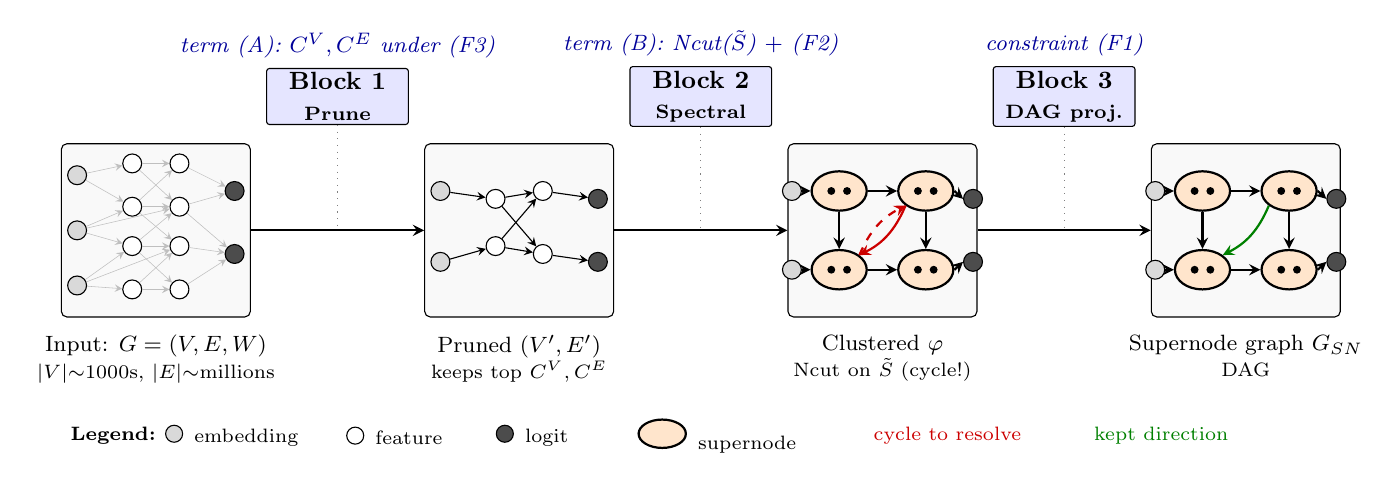
\begin{tikzpicture}[
  font=\small,
  >=stealth,
  node distance=2mm,
  graphbox/.style={draw, rounded corners=2pt, minimum width=24mm,
                   minimum height=22mm, align=center, inner sep=2pt,
                   fill=gray!5},
  blocklabel/.style={draw, rounded corners=1pt, fill=blue!10,
                     minimum width=18mm, minimum height=5.5mm,
                     font=\small\bfseries, align=center,
                     inner sep=1.5pt},
  termlabel/.style={font=\footnotesize\itshape, align=center,
                    text=blue!60!black, inner sep=1pt},
  arrow/.style={->, thick, >=stealth},
  fnode/.style={circle, draw, inner sep=0pt, minimum size=2.4mm,
                fill=white},
  enode/.style={circle, draw, inner sep=0pt, minimum size=2.4mm,
                fill=gray!30},
  lnode/.style={circle, draw, inner sep=0pt, minimum size=2.4mm,
                fill=black!70, text=white, font=\tiny},
  snode/.style={ellipse, draw, thick, inner sep=1pt,
                minimum width=10mm, minimum height=6mm,
                fill=orange!20},
  caplabel/.style={font=\footnotesize, align=center}
]

% =========================================================
% STAGE 1: Input attribution graph G
% =========================================================
\node[graphbox] (G) at (0,0) {};
\node[enode] (e1) at (-1.0, 0.7) {};
\node[enode] (e2) at (-1.0, 0.0) {};
\node[enode] (e3) at (-1.0,-0.7) {};
\node[fnode] (f1) at (-0.3, 0.85) {};
\node[fnode] (f2) at (-0.3, 0.3)  {};
\node[fnode] (f3) at (-0.3,-0.2)  {};
\node[fnode] (f4) at (-0.3,-0.75) {};
\node[fnode] (f5) at ( 0.3, 0.85) {};
\node[fnode] (f6) at ( 0.3, 0.3)  {};
\node[fnode] (f7) at ( 0.3,-0.2)  {};
\node[fnode] (f8) at ( 0.3,-0.75) {};
\node[lnode] (l1) at ( 1.0, 0.5) {};
\node[lnode] (l2) at ( 1.0,-0.3) {};
\foreach \s/\t in {e1/f1, e1/f2, e2/f2, e2/f3, e2/f6, e3/f4, e3/f7,
                   e3/f3, f1/f5, f2/f5, f2/f6, f3/f6, f3/f7, f4/f7,
                   f4/f8, f5/l1, f6/l1, f6/l2, f7/l2, f8/l2, f1/f6,
                   f2/f7, f3/f8}
  \draw[->, gray!50, line width=0.2pt] (\s) -- (\t);
\node[caplabel, below=1mm of G.south]
  {Input: $G=(V,E,W)$\\\scriptsize $|V|$$\sim$1000s, $|E|$$\sim$millions};

% =========================================================
% STAGE 2: Pruned graph G' after Block 1
% =========================================================
\node[graphbox, right=22mm of G] (Gp) {};
\node[enode] (pe1) at ($(Gp)+(-1.0, 0.5)$) {};
\node[enode] (pe2) at ($(Gp)+(-1.0,-0.4)$) {};
\node[fnode] (pf2) at ($(Gp)+(-0.3, 0.4)$) {};
\node[fnode] (pf3) at ($(Gp)+(-0.3,-0.2)$) {};
\node[fnode] (pf6) at ($(Gp)+( 0.3, 0.5)$) {};
\node[fnode] (pf7) at ($(Gp)+( 0.3,-0.3)$) {};
\node[lnode] (pl1) at ($(Gp)+( 1.0, 0.4)$) {};
\node[lnode] (pl2) at ($(Gp)+( 1.0,-0.4)$) {};
\foreach \s/\t in {pe1/pf2, pe2/pf3, pf2/pf6, pf3/pf6, pf3/pf7,
                   pf6/pl1, pf7/pl2, pf2/pf7}
  \draw[->, black, line width=0.4pt] (\s) -- (\t);
\node[caplabel, below=1mm of Gp.south]
  {Pruned $(V',E')$\\\scriptsize keeps top $C^V,C^E$};

% =========================================================
% STAGE 3: Clustered graph after Block 2 (cycle present)
% =========================================================
\node[graphbox, right=22mm of Gp] (Gc) {};

% Supernodes
\node[snode, minimum width=7mm, minimum height=5mm]
  (s1) at ($(Gc)+(-0.55, 0.5)$) {};
\node[snode, minimum width=7mm, minimum height=5mm]
  (s2) at ($(Gc)+(-0.55,-0.5)$) {};
\node[snode, minimum width=7mm, minimum height=5mm]
  (s3) at ($(Gc)+( 0.55, 0.5)$) {};
\node[snode, minimum width=7mm, minimum height=5mm]
  (s4) at ($(Gc)+( 0.55,-0.5)$) {};

% Embedding/logit columns (named so we can draw edges to/from them)
\node[enode] (ec1) at ($(Gc)+(-1.15, 0.5)$) {};
\node[enode] (ec2) at ($(Gc)+(-1.15,-0.5)$) {};
\node[lnode] (lc1) at ($(Gc)+( 1.15, 0.4)$) {};
\node[lnode] (lc2) at ($(Gc)+( 1.15,-0.4)$) {};

% Feature dots inside each supernode
\foreach \dx/\dy in {-0.65/0.5, -0.45/0.5}
  \fill[black] ($(Gc)+(\dx,\dy)$) circle (0.5mm);
\foreach \dx/\dy in {-0.65/-0.5, -0.45/-0.5}
  \fill[black] ($(Gc)+(\dx,\dy)$) circle (0.5mm);
\foreach \dx/\dy in {0.45/0.5, 0.65/0.5}
  \fill[black] ($(Gc)+(\dx,\dy)$) circle (0.5mm);
\foreach \dx/\dy in {0.45/-0.5, 0.65/-0.5}
  \fill[black] ($(Gc)+(\dx,\dy)$) circle (0.5mm);

% Boundary edges: embeddings -> left supernodes, right supernodes -> logits
\draw[->, thick] (ec1.east) -- (s1.west);
\draw[->, thick] (ec2.east) -- (s2.west);
\draw[->, thick] (s3.east)  -- (lc1.west);
\draw[->, thick] (s4.east)  -- (lc2.west);

% Inter-supernode directed edges
\draw[->, thick] (s1.east)  -- (s3.west);
\draw[->, thick] (s2.east)  -- (s4.west);
\draw[->, thick] (s1.south) -- (s2.north);
\draw[->, thick] (s3.south) -- (s4.north);

% Highlighted 2-cycle (red): one direction solid, opposite dashed
\draw[->, thick, red!80!black]
  (s3.south west) to[bend left=20] (s2.north east);
\draw[->, thick, red!80!black, dashed]
  (s2.north east) to[bend left=20] (s3.south west);

\node[caplabel, below=1mm of Gc.south]
  {Clustered $\varphi$\\\scriptsize Ncut on $\tilde S$ (cycle!)};

% =========================================================
% STAGE 4: Final supernode graph (DAG)
% =========================================================
\node[graphbox, right=22mm of Gc] (Gf) {};

\node[snode, minimum width=7mm, minimum height=5mm]
  (fs1) at ($(Gf)+(-0.55, 0.5)$) {};
\node[snode, minimum width=7mm, minimum height=5mm]
  (fs2) at ($(Gf)+(-0.55,-0.5)$) {};
\node[snode, minimum width=7mm, minimum height=5mm]
  (fs3) at ($(Gf)+( 0.55, 0.5)$) {};
\node[snode, minimum width=7mm, minimum height=5mm]
  (fs4) at ($(Gf)+( 0.55,-0.5)$) {};

\node[enode] (ef1) at ($(Gf)+(-1.15, 0.5)$) {};
\node[enode] (ef2) at ($(Gf)+(-1.15,-0.5)$) {};
\node[lnode] (lf1) at ($(Gf)+( 1.15, 0.4)$) {};
\node[lnode] (lf2) at ($(Gf)+( 1.15,-0.4)$) {};

\foreach \dx/\dy in {-0.65/0.5, -0.45/0.5}
  \fill[black] ($(Gf)+(\dx,\dy)$) circle (0.5mm);
\foreach \dx/\dy in {-0.65/-0.5, -0.45/-0.5}
  \fill[black] ($(Gf)+(\dx,\dy)$) circle (0.5mm);
\foreach \dx/\dy in {0.45/0.5, 0.65/0.5}
  \fill[black] ($(Gf)+(\dx,\dy)$) circle (0.5mm);
\foreach \dx/\dy in {0.45/-0.5, 0.65/-0.5}
  \fill[black] ($(Gf)+(\dx,\dy)$) circle (0.5mm);

% Boundary edges
\draw[->, thick] (ef1.east) -- (fs1.west);
\draw[->, thick] (ef2.east) -- (fs2.west);
\draw[->, thick] (fs3.east) -- (lf1.west);
\draw[->, thick] (fs4.east) -- (lf2.west);

% Inter-supernode edges
\draw[->, thick] (fs1.east)  -- (fs3.west);
\draw[->, thick] (fs2.east)  -- (fs4.west);
\draw[->, thick] (fs1.south) -- (fs2.north);
\draw[->, thick] (fs3.south) -- (fs4.north);

% Resolved cycle: only one direction retained
\draw[->, thick, darkgreen]
  (fs3.south west) to[bend left=20] (fs2.north east);

\node[caplabel, below=1mm of Gf.south]
  {Supernode graph $G_{SN}$\\\scriptsize DAG};
% =========================================================
% PIPELINE ARROWS (drawn first; sit below the labels visually)
% =========================================================
\draw[arrow] (G.east)  -- (Gp.west);
\draw[arrow] (Gp.east) -- (Gc.west);
\draw[arrow] (Gc.east) -- (Gf.west);

% =========================================================
% BLOCK + TERM LABELS, stacked ABOVE the graph boxes so they
% don't overlap arrows or boxes.
% Graph boxes top ~ y = +1.1; place stack starting at y = +1.7.
% =========================================================
\node[blocklabel] (b1) at ($(G.east)!0.5!(Gp.west) + (0, 1.7)$)
  {Block 1\\\scriptsize Prune};
\node[termlabel, above=0.8mm of b1]
  {term (A): $C^V, C^E$ under (F3)};

\node[blocklabel] (b2) at ($(Gp.east)!0.5!(Gc.west) + (0, 1.7)$)
  {Block 2\\\scriptsize Spectral};
\node[termlabel, above=0.8mm of b2]
  {term (B): Ncut($\tilde S$) $+$ (F2)};

\node[blocklabel] (b3) at ($(Gc.east)!0.5!(Gf.west) + (0, 1.7)$)
  {Block 3\\\scriptsize DAG proj.};
\node[termlabel, above=0.8mm of b3]
  {constraint (F1)};

% Tiny vertical tick from each block label down to its arrow,
% so the reader sees the label "applies to" that arrow.
\draw[dotted, gray] (b1.south) -- ($(G.east)!0.5!(Gp.west)$);
\draw[dotted, gray] (b2.south) -- ($(Gp.east)!0.5!(Gc.west)$);
\draw[dotted, gray] (b3.south) -- ($(Gc.east)!0.5!(Gf.west)$);

% =========================================================
% LEGEND at bottom
% =========================================================
\node[anchor=west, font=\scriptsize] at ($(G.south west)+(0,-1.5)$)
  {\textbf{Legend:}};
\node[anchor=west, font=\scriptsize] at ($(G.south west)+(1.2,-1.5)$)
  {\tikz\node[enode, scale=0.9]{};\, embedding};
\node[anchor=west, font=\scriptsize] at ($(G.south west)+(3.5,-1.5)$)
  {\tikz\node[fnode, scale=0.9]{};\, feature};
\node[anchor=west, font=\scriptsize] at ($(G.south west)+(5.4,-1.5)$)
  {\tikz\node[lnode, scale=0.9]{};\, logit};
\node[anchor=west, font=\scriptsize] at ($(G.south west)+(7.2,-1.5)$)
  {\tikz\node[snode, scale=0.6]{};\, supernode};
\node[anchor=west, font=\scriptsize, text=red!80!black]
  at ($(G.south west)+(10.2,-1.5)$) {cycle to resolve};
\node[anchor=west, font=\scriptsize, text=darkgreen]
  at ($(G.south west)+(13.0,-1.5)$) {kept direction};

\end{tikzpicture}
\caption{The ASG pipeline as block-coordinate descent on
$\mathcal{J}_K$. \textbf{Block~1} prunes $(V', E')$ by
cumulative-mass thresholding on the combined evidence scores
$C^V, C^E$, solving term~(A) under the budget constraint (F3) as a
unit-cost knapsack. \textbf{Block~2} partitions the surviving
features by spectral clustering on the bidirectional affinity
$\tilde S$, solving term~(B) at fixed $(V', E')$ via the
Shi--Malik relaxation and absorbing layer locality (F2) through the
exponential decay in $\tilde S$. \textbf{Block~3} restores the DAG
constraint (F1) by per-pair direction selection (eliminating the
2-cycle highlighted in red) followed by SCC-split-at-widest-span.
The coupling between blocks is one-directional within a sweep
($(V', E') \to \tilde S \to \varphi$), so the single forward sweep
is a fixed point of the coordinate iteration. Granularity $K$ is
selected externally over the grid $\mathcal{K}$ (not shown).}
\label{fig:pipeline}
\end{figure*}

$\mathcal{J}_K$ is jointly intractable, so we decompose by variable
(Figure~\ref{fig:pipeline}). The dependency graph between terms and
variables is acyclic: term~(A) sees only $(V', E')$; term~(B)
couples $(V', E')$ and $\varphi$ but only through
$\tilde S(V', E')$, which is fixed once $(V', E')$ are. This gives
a two-block coordinate descent in the variables. A third step is
required by~(F1), which is combinatorial in $\varphi$ and admits no
smooth penalty compatible with the Ncut relaxation; it must be
enforced as a feasibility projection after clustering.

We emphasize that a single forward sweep is \emph{not} a fixed
point of coordinate descent on $\mathcal{J}_K$. Block~3 modifies
$\varphi$ to restore~(F1), and term~(B) depends on $\varphi$, so
the post-projection partition is in general suboptimal for
$\Ncut(\varphi; \tilde S)$ relative to the Block~2 output. What
does hold is weaker: the coupling among \emph{terms (A) and (B)
before projection} is one-directional
($(V', E') \to \tilde S \to \varphi$), so Blocks~1--2 form an exact
forward pass on the relaxed problem (without~F1), and Block~3 is a
feasibility projection onto the DAG constraint. Iterating the sweep
could in principle decrease $\mathcal{J}_K$ further by re-clustering
against the projected $\varphi$; we do not do so, treating the
single sweep as a deliberate computational simplification rather
than a fixed-point property.

\paragraph{Block 1: pruning.}
Hold $\varphi$ uncommitted and drop term~(B). The remaining
subproblem in $(V', E')$ is a unit-cost knapsack on $C^V$ and $C^E$
under budget (F3), with housekeeping cleanup. The exact greedy
solver---sort by score, take the prefix that fills the budget---is
implemented as cumulative-mass thresholding at rank percentiles
$\eta_V, \eta_E$. Edge scores are recomputed on the node-pruned
graph since $\text{Inf}_{uv}, \text{Rel}_{uv}$ depend on surviving
edges; this is a greedy-on-greedy approximation when the two
knapsacks couple through the recomputation. Full procedure and
threshold derivation in Appendix~\ref{app:method}.D.

\paragraph{Block 2: clustering.}
Substitute the pruned graph into $\tilde S$, drop (F1), and absorb
(F2) into the affinity. The remaining problem is
$\min_\varphi \Ncut(\varphi; \tilde S)$ at $|\pi(\varphi)| = K$.
We solve it by Shi--Malik spectral
relaxation~\cite{shi2000normalized, von2007tutorial}: project onto
the bottom-$K$ eigenvectors of the symmetric normalized Laplacian
of $\tilde S$, then discretize via $K$-means. The volume
denominators of Ncut provide implicit balance, which is how (C3)
is handled in this framework; a small $\varepsilon$-clamp on
$\tilde S$ keeps the Laplacian connected.

\paragraph{Block 3: DAG projection.}
The output of Block~2 may violate (F1). We restore it in two steps.
(i) \emph{Per-pair direction.} For each unordered cluster pair, let
$M(S_k \!\to\! S_l) = \sum_{i \in S_k, j \in S_l} W'_{ij}$ and
retain only the direction with strictly greater absolute mass; this
optimally eliminates every 2-cycle. (ii) \emph{SCC-split.} For each
strongly connected component of size $\ge 2$, split the cluster
with the widest layer span at its median layer; each split
increases $|\pi(\varphi)|$ by one. Repeat until no SCCs remain.
Termination, ordering rationale, and the layer-locality descent
argument are in Appendix~\ref{app:method}.E. Block~3 thus does
double duty: it enforces (F1) and simultaneously tightens (F2) by
reducing the layer span of every cluster it splits.

\paragraph{Optimality.}
Block~1 is exact for each of its two subproblems (unit-cost
knapsack) but not jointly optimal in $(V', E')$ due to the
edge-score recomputation coupling
(Proposition~\ref{prop:block1}). Block~2 inherits the higher-order
Cheeger bound for spectral Ncut relaxation
(Proposition~\ref{prop:block2}). Block~3 is a feasibility
projection with no approximation guarantee against minimum-mass DAG
repair (the latter being Min-Feedback-Arc-Set on the cluster
graph). No joint bound on $\mathcal{J}_K$ is claimed. Formal
statements in Appendix~\ref{app:method}.F.
Table~\ref{tab:obj-algo} summarizes the mapping.

\begin{table}[t]
\centering
\caption{Mapping from objective components to algorithm steps.}
\label{tab:obj-algo}
\footnotesize
\begin{tabular}{@{}lll@{}}
\toprule
\textbf{Component} & \textbf{Step} & \textbf{Optimality}\\
\midrule
Term (A) + F3       & Cumulative-mass pruning & Per-subproblem exact \\
                    &                         & (Prop.~\ref{prop:block1}) \\
Term (B), fixed $K$ & Spectral + $K$-means    & Higher-order Cheeger \\
F2 (in term B)      & $e^{-\lambda \Delta_{ij}}$ decay & Soft (Lagrangian) \\
Constraint F1       & Direction + SCC-split   & Feasibility only \\
Housekeeping        & Dangling cleanup        & Exact \\
C3 (no term)        & Implicit in Ncut volumes & Implicit \\
$K$ selection       & Grid search + $\Psi$ (\S\ref{sec:k-selection}) & Heuristic \\
\bottomrule
\end{tabular}
\end{table}

\begin{algorithm}[h]
\caption{Block-coordinate strategy on $\mathcal{J}_K$}
\label{alg:asg}
\begin{algorithmic}[1]
\REQUIRE Attribution graph $G$;
hyperparameters $(\eta_V, \eta_E, \alpha, \lambda, F_{\text{mean}})$;
grid $\mathcal{K}$; criterion $\Psi$
\ENSURE Supernode graph $G_{SN}$
\STATE $(V', E') \gets \textsc{Prune}(G, \eta_V, \eta_E, \alpha)$
       \COMMENT{Block 1; Appendix~\ref{app:method}.D}
\STATE Build $\tilde S(V', E')$ via
       Eqs.~\eqref{eq:signatures}--\eqref{eq:Stilde}
\FOR{$K \in \mathcal{K}$}
  \STATE $\varphi^{(K)} \gets
         \textsc{SpectralCluster}(\tilde S, K)$
         \COMMENT{Block 2}
  \STATE $\varphi^{(K)} \gets
         \textsc{PerPairDirection}(\varphi^{(K)}, W')$
         \COMMENT{Block 3, step (i)}
  \WHILE{$\exists$ SCC of size $\ge 2$ in $G_{SN}(\varphi^{(K)})$}
    \STATE split widest-span cluster at its median layer
    \COMMENT{Block 3, step (ii)}
  \ENDWHILE
  \STATE $\psi_K \gets \Psi(G_{SN}(\varphi^{(K)}))$
\ENDFOR
\STATE $K^\star \gets \argmax_{K \in \mathcal{K}} \psi_K$
\RETURN $G_{SN}(\varphi^{(K^\star)})$
\end{algorithmic}
\end{algorithm}

\subsection{Granularity selection}\label{sec:k-selection}

$K$ is not optimized inside $\mathcal{J}_K$; it is selected by an
external grid search over a finite set $\mathcal{K}$, using a
criterion $\Psi$ computed on the resulting supernode graph. We use
the unweighted mean of five graph-theoretic quality measures
(back-edge fraction, internal independence, size entropy,
opposing-sign fraction, output-direction cosine gap), each oriented
so larger is better and standardized to $[0,1]$ before averaging.
Definitions and targeting (which criterion each measure probes) are
in Appendix~\ref{app:method}.G. The chosen granularity is
\begin{equation}
K^\star = \argmax_{K \in \mathcal{K}} \Psi(G_{SN}^{(K)}), \quad
\Psi = \tfrac{1}{|\mathcal{M}|}\sum_{m \in \mathcal{M}}\psi^{(m)}_K.
\label{eq:K-star}
\end{equation}
We use $\mathcal{K} = \{\lfloor n/2 \rfloor, \lfloor n/3 \rfloor\}$
with $n = |V'_{\text{feat}}|$, so Algorithm~\ref{alg:asg}'s outer
loop runs Blocks~2--3 twice per graph. $\Psi$ is evaluated on the
post-projection graph, which accounts for the slack from
SCC-splits inflating $|\pi(\varphi)|$ above $K$.

\paragraph{Relationship to $\mathcal{J}_K$.}
$\Psi$ is not an independent quality criterion: of its five
constituents, three (internal independence, opposing-sign fraction,
output-direction cosine gap) target (C2), one (back-edge fraction)
targets (F1), and one (size entropy) targets (C3). Term~(B) of
$\mathcal{J}_K$ operationalizes (C2), so $\Psi$ partly re-measures
what the inner objective already optimizes, on a different
functional form (graph statistics rather than Ncut). The
justification for using $\Psi$ rather than $\mathcal{J}_K$ itself
for $K$-selection is twofold: (i)~$\mathcal{J}_K$ values are not
comparable across $K$ because the Ncut scale depends on the number
of clusters, and (ii)~$\Psi$ scores the post-projection graph,
capturing the slack from SCC-splits.

A more principled choice of $\Psi$ would be downstream
interventional measures---specifically the edge-level Spearman
correlation $\rho_{\text{edge}}$ and the per-feature cosine gap
$\kappa_{\text{intra}} - \kappa_{\text{inter}}$ defined in
Section~\ref{sec:causal-validation}. We use the graph-theoretic mean
because it is cheap to compute on every
$(K, F_{\text{mean}}, \lambda)$ configuration in the sweep, whereas
the interventional measures require forward passes through the
transcoder substrate per ablation and are tractable only at
evaluation time on a fixed configuration. Replacing $\Psi$ with a
learned criterion calibrated against the interventional measures is
a natural extension (Section~\ref{sec:limitations}).

\section{Experiments}\label{sec:exp}

We evaluate the block-coordinate solver against three $K$-matched
baselines on attribution graphs from Gemma-2-2B.

\subsection{Setup}

\paragraph{Datasets.}
We evaluate on attribution graphs from Gemma-2-2B on
\emph{analogies prompts} of the form ``The saying goes: A is to B as
C is to,'' testing whether the model recovers the relation between
A and B and applies it to C. We report on $N=55$ pruned attribution
graphs. Results on a multihop reasoning dataset are qualitatively
consistent and deferred to Appendix~\ref{app:multihop}.

\paragraph{Baselines.}
All baselines operate on the same Block~1 output as our solver and
are forced to produce the same $K$:
\begin{itemize}[leftmargin=*,topsep=2pt,itemsep=1pt]
\item \textbf{Modularity}: greedy modularity maximization on the
symmetrized weighted adjacency, constrained to $K$ communities. Blind
to edge direction.
\item \textbf{Spectral-RBF}: spectral clustering with an RBF kernel
over per-feature bidirectional adjacency rows. Recovers local
geometry without using the attribution-weighted similarity of
Eq.~\eqref{eq:Stilde}.
\item \textbf{K-means}: K-means on the same bidirectional adjacency
features. The simplest non-trivial partition baseline.
\end{itemize}

\paragraph{Quality measures.}
The five measures of Section~\ref{sec:k-selection}: back-edge fraction
($\downarrow$), internal independence ($\uparrow$), size entropy
($\uparrow$), opposing-sign fraction ($\downarrow$), and
output-direction cosine gap ($\uparrow$). None of the measures uses
$\tilde S$, so each is independent of the affinity that drives our
clustering step.

\paragraph{Sweeps.}
We sweep $K \in \{\lfloor n/2 \rfloor, \lfloor n/3 \rfloor\}$, the
mean operator $F_{\text{mean}} \in \{\text{arith, harm, geo}\}$, and
the layer-span dual $\lambda \in \{0.0, 0.1, \ldots, 1.0\}$. We
report ASG numbers averaged over $\lambda$ and shown separately for
each mean operator.

\subsection{Results}

Table~\ref{tab:main} summarizes performance. The three ASG variants
together dominate all causal-coherence measures. At every $K$,
\textsc{ASG-arith} records 3.6--9.2$\times$ fewer back-edges than
the best baseline (Table~\ref{tab:main}) and ranks first on internal
independence, while \textsc{ASG-harm} and \textsc{ASG-geo}
essentially eliminate opposing-sign pairs (0.008--0.086 vs
0.235--0.400 for baselines) and push intra-supernode output
directions into near-unit alignment (cosine gap 0.96--0.99 vs
$-0.04$ to 0.44).

\paragraph{Reading by objective term.}
The mean operator $F_{\text{mean}}$ acts on term (B) through $\tilde S$.
Arithmetic preserves more in/out structural signal and so wins the
structural measures (back-edge, independence); harmonic and geometric
sharpen the similarity by penalizing pairs weak on either side,
producing tighter directionally-consistent clusters at the cost of a
small rise in back-edges. Modularity wins size entropy by virtue of
its balance-favoring objective but loses every causal-coherence
measure---a direct consequence of being undirected (it sees no
constraint (F1)).

\paragraph{Internal independence saturates.}
Internal independence is above 0.90 across all methods on this
dataset and is not discriminative; we retain it for completeness but
caution against treating it as a primary signal in the criterion.

\begin{table*}[t]
\centering
\caption{Quality measures on the analogies dataset ($N=55$ pruned
graphs). ASG rows show the spectral variant averaged over
$\lambda \in \{0.0, \ldots, 1.0\}$ at each choice of mean operator.
Bold marks the best entry per (measure, $K$) cell.}
\label{tab:main}
\small
\begin{tabular}{@{}lcccccc@{}}
\toprule
\textbf{Method} & $K$ & back-edge $\downarrow$ & indep.\ $\uparrow$ & size-H $\uparrow$ & opp-sign $\downarrow$ & out-dir gap $\uparrow$ \\
\midrule
\textsc{ASG-arith} & $n/2$ & \textbf{0.015} & \textbf{0.980} & 0.928 & 0.104 & 0.735 \\
\textsc{ASG-harm}  & $n/2$ & 0.031 & 0.975 & 0.918 & \textbf{0.008} & \textbf{0.970} \\
\textsc{ASG-geo}   & $n/2$ & 0.030 & 0.975 & 0.920 & 0.011 & 0.962 \\
Modularity         & $n/2$ & 0.132 & 0.941 & \textbf{0.989} & 0.400 & $-0.036$ \\
Spectral-RBF       & $n/2$ & 0.138 & 0.958 & 0.841 & 0.252 & 0.430 \\
K-means            & $n/2$ & 0.111 & 0.969 & 0.895 & 0.235 & 0.436 \\
\midrule
\textsc{ASG-arith} & $n/3$ & \textbf{0.039} & \textbf{0.946} & 0.898 & 0.172 & 0.756 \\
\textsc{ASG-harm}  & $n/3$ & 0.064 & 0.941 & 0.906 & \textbf{0.085} & \textbf{0.987} \\
\textsc{ASG-geo}   & $n/3$ & 0.063 & 0.942 & 0.908 & 0.086 & 0.982 \\
Modularity         & $n/3$ & 0.194 & 0.906 & \textbf{0.978} & 0.373 & 0.048 \\
Spectral-RBF       & $n/3$ & 0.232 & 0.922 & 0.793 & 0.325 & 0.203 \\
K-means            & $n/3$ & 0.140 & 0.931 & 0.827 & 0.277 & 0.360 \\
\bottomrule
\end{tabular}
\end{table*}

\subsection{Granularity selection in practice}

Computing the criterion $\Psi$ of Eq.~\eqref{eq:K-star} on each row
of Table~\ref{tab:main} (with cost-style measures negated and all
measures standardized to $[0,1]$) and averaging selects
\textsc{ASG-harm} or \textsc{ASG-geo} at $K=n/2$ as the maximum,
consistent with their dominance on the directional measures despite
slightly higher back-edge fractions. This validates the criterion as
a usable proxy for picking $K^\star$: it favors the partition that
best balances the causal-coherence measures (the ones the objective
$\mathcal{J}_K$ targets through term (B)) without being dragged
around by the saturated internal-independence column.

\subsection{Causal validation via supernode-level ablation}\label{sec:causal-validation}

The measures of Table~\ref{tab:main} are graph-theoretic: they
evaluate the supernode partition through the (already-computed)
attribution graph. To verify the partition is also causally
meaningful, we ablate features through the cross-layer transcoder
substrate, clamping each feature's post-encoder activation to zero
and propagating the modified state.

\paragraph{Edge-level test.}
For each feature-supernode pair $(S_A, S_B)$ with
$W^{SN}(S_A \to S_B) > 0$, we record the downstream activation-drop
ratio $r_{A \to B} = \bar z^{S_A}(S_B) / (\bar z^0(S_B) + \varepsilon)$.
A causally faithful supernode graph should yield positive Spearman
correlation between supernode edge weights and downstream drops:
\begin{equation}
\rho_{\text{edge}} = \mathrm{Spearman}\bigl(W^{SN}(S_A \to S_B),\; 1 - r_{A \to B}\bigr).
\label{eq:rho-edge}
\end{equation}
This probes whether the supernode edges---defined as aggregated
attribution mass---predict actual causal effects, which is the
strongest interventional test of term (B) we can construct from the
partition alone.

\paragraph{Per-feature test.}
For each feature $f \in S$, we ablate $f$ in isolation and record the
last-position logit perturbation $\Delta_f$. We compute the
intra-supernode mean pairwise cosine $\kappa_{\text{intra}}(S)$ and
average over supernodes; the cross-supernode baseline $\kappa_{\text{inter}}$
is the mean cosine over $M=1000$ random feature pairs from different
supernodes. A high gap $\kappa_{\text{intra}} - \kappa_{\text{inter}}$
indicates that grouped features push the logit distribution in
genuinely similar directions---an interventional counterpart to the
output-direction cosine measure of Section~\ref{sec:k-selection}.

\section{Limitations and Future Work}\label{sec:limitations}

The block-coordinate strategy makes several approximations that
admit natural improvements within our framework:

\paragraph{Block 1.} Greedy is exact for fractional knapsack but the
sequential node-then-edge decomposition is only an approximation when
the two knapsacks couple through the $C^E$ recomputation. A joint
formulation over $(V', E')$ would tighten this.

\paragraph{Block 2.} The Shi--Malik relaxation is a known
approximation with bounded conductance gap. An augmented-Lagrangian
treatment of the layer-span constraint, replacing the soft
$e^{-\lambda \Delta}$ with explicit constraint enforcement, would
tighten the dual.

\paragraph{Block 3.} The greedy SCC-split has no global optimality
guarantee. Replacing it with min-cost feedback arc set on the cluster
graph would optimally repair the DAG constraint at minimum mass loss,
and is the largest improvement headroom in the pipeline.

\paragraph{Single-sweep coordinate descent.}
The pipeline is a single forward sweep rather than an iterated
coordinate descent. Block~3's modification of $\varphi$ takes the
partition off the Block~2 optimum, so iterating Blocks~2--3 (with
Block~1 frozen) could decrease $\mathcal{J}_K$ further. We do not
characterize the size of this gap.

\paragraph{Granularity criterion.} The mean of standardized quality
measures gives equal weight to each measure. A learned criterion,
calibrated against downstream interventional tests
($\rho_{\text{edge}}$, $\kappa_{\text{intra}} - \kappa_{\text{inter}}$),
would target the partition's actual causal utility rather than
graph-theoretic proxies.

\paragraph{Attribution backend.} The framework inherits limitations
from the underlying attribution method: attribution quality depends
on transcoder fidelity and may be biased toward high-magnitude edges
that are not causally primary. Stronger causal validation across
model families beyond Gemma is needed.

\section{Conclusion}

We formulated attribution-graph summarization as a single
constrained optimization problem $\mathcal{J}_K$ over the pruned
subgraph and supernode partition, with two terms tied to
faithfulness and coherence (plus implicit balance from the cut
volumes), and hard constraints encoding DAG integrity, layer span,
and a complexity budget. The granularity $K$ is selected by external
grid search under the mean of standardized supernode-graph quality
measures. We then showed that the standard ASG pipeline---
rank-percentile pruning, spectral clustering on a layer-decayed
bidirectional affinity, and DAG projection---is a block-coordinate
descent strategy on this objective, with one principled relaxation
or projection per block. This framing makes each hyperparameter the
dual of a constraint or a structural choice about evidence pooling,
locates the algorithm's optimality gaps (spectral relaxation, greedy
DAG repair, single-sweep coordinate descent), and points to concrete
improvements in each block.

\bibliography{ref}
\bibliographystyle{acl_natbib}


\appendix
\appendix

\section{Method Details}\label{app:method}

This appendix contains the derivations and procedures referenced in
Sections~\ref{sec:setup}--\ref{sec:solution}. Subsections are
cross-referenced from the main text as
``Appendix~\ref{app:method}.1''--``Appendix~\ref{app:method}.6.''

\subsection*{A.1 Flow quantities (Inf and Rel)}\label{app:flow}

Defining column- and row-normalized weight matrices
$W^{\text{in}}_{ij} = |W_{ij}|/\sum_k |W_{kj}|$ and
$W^{\text{out}}_{ij} = |W_{ij}|/\sum_k |W_{ik}|$, the Neumann series
$\sum_t (W^{\text{in}})^t$ converges on the DAG, giving
$\text{Inf} = \ell^\top (I - (W^{\text{in}})^\top)^{-1}$ and
$\text{Rel} = \tau^\top (I - W^{\text{out}})^{-1}$. Edge-level
analogues are $\text{Inf}_{uv} = \text{Inf}_v W^{\text{in}}_{uv}$
and $\text{Rel}_{uv} = \text{Rel}_u W^{\text{out}}_{uv}$. Rank
percentiles are $\widehat{s}_u = |\{v : s_v < s_u\}|/(N-1)$.
\emph{Discussion of DAG convergence, edge-level decomposition, and
the rank-percentile transform.}

\subsection*{A.2. Combined evidence: pooling choice}\label{app:pooling}

Comparison of arithmetic, harmonic, and geometric pooling for
$C^V_u$. The geometric mean is the log-linear pool of independent
rank evidences~\cite{genest1986combining}; additive pooling allows
one strong axis to mask a weak one and is therefore unsuitable for
C1. Edge-score recomputation rationale on the node-pruned graph.

\subsection*{A.3. Bidirectional affinity: matrix form and pairing}\label{app:affinity}

Equivalent matrix form of the signature-vector definition:
\begin{align}
S^{\text{out}} = \mathrm{ReLU}\,\mathrm{CosNorm}(W' \,\mathrm{diag}(\text{Inf})\, W'^\top)\\
S^{\text{in}}  = \mathrm{ReLU}\,\mathrm{CosNorm}(W'^\top \,\mathrm{diag}(\text{Rel})\, W'),
\end{align}
where $\mathrm{CosNorm}(M)_{ij} = M_{ij}/\sqrt{M_{ii}M_{jj}}$.
Geometry argument for the Inf/Rel pairing: targets of outgoing edges
are downstream and so weighted by downstream importance ($\text{Inf}$);
sources of incoming edges are upstream and so weighted by upstream
importance ($\text{Rel}$); any other pairing weights an axis by an
importance score irrelevant to that axis. Discussion of the
$F_{\text{mean}}$ choice (arithmetic, harmonic, geometric).

\subsection*{A.4. Block 1: pruning algorithm}\label{app:block1}

Cumulative-mass thresholding rule:
\begin{align}
M_\eta(C) = \{u : C_u \ge C_{(t)}\}, \\
t = \min\{k : \tfrac{\sum_{j \le k} C_{(j)}}{\sum_j C_{(j)}} \ge \eta\},
\end{align}
with $C_{(j)}$ the $j$-th largest score. Duality between
$(\eta_V, \eta_E)$ and the primal budget $(B, \beta)$ is monotonic:
for fixed score distribution, increasing $\eta$ enlarges the kept
set, which relaxes the budget constraint. Sequential node-then-edge
application, dangling-node cleanup loop, and full pseudocode (former
Algorithm~1).

\subsection*{A.5. Block 3: DAG projection procedure}\label{app:block3}

Per-pair direction selection: optimality for 2-cycle elimination.
SCC-split-at-widest-span: termination in at most $|V'_{\text{feat}}|$
splits (each increases $|\pi(\varphi)|$ by one, bounded by the
feature count); justification for splitting at the median (minimizes
resulting maximum layer span); justification for selecting the
widest-span cluster first (steepest layer-locality descent per
split). Full procedure pseudocode.

\subsection*{A.6. Optimality remarks}\label{app:optimality}

\begin{proposition}[Block 1]\label{prop:block1}
For fixed $(\eta_V, \eta_E)$, the node-pruning subproblem
$\max_{V' \subseteq V} \sum_{u \in V'} C^V_u$ subject to
$|V'| \le B_V$ is solved exactly by sorting on $C^V$ and taking the
top-mass prefix (unit-cost knapsack, hence trivially exact). The
edge-pruning subproblem
$\max_{E' \subseteq E \cap (V' \times V')} \sum_{(u,v) \in E'} C^E_{uv}$
subject to $|E'| \le B_E$, on the node-pruned graph, is likewise
solved exactly by cumulative-mass thresholding. The sequential
composition (node-prune, then edge-prune on the result) is
\emph{not} jointly optimal in $(V', E')$, because $C^E_{uv}$ depends
on the surviving edge set through the recomputation of
$\text{Inf}_{uv}$ and $\text{Rel}_{uv}$ on the node-pruned graph; a
node removed in the first step may carry edges whose joint mass
would have exceeded that of edges kept in the second step under the
original graph's flow quantities. The conditional optimality of the
sequential procedure is the standard guarantee for greedy-on-greedy
decompositions of coupled knapsacks; a joint LP relaxation would
tighten this and is the natural improvement headroom for Block~1.
\end{proposition}

\begin{proposition}[Block 2]\label{prop:block2}
Let $\varphi^\star$ minimize $\Ncut(\,\cdot\,; \tilde S)$ over
partitions of $V'_{\text{feat}}$ into $K$ nonempty clusters, and let
$\varphi_{\text{spec}}$ be the partition recovered by Shi--Malik
spectral relaxation followed by $K$-means rounding on the bottom-$K$
eigenvectors of the symmetric normalized Laplacian of $\tilde S$.
Then the higher-order Cheeger inequalities of
\cite{lee2014multiway, louis2012many} give
\begin{equation}
\Ncut(\varphi_{\text{spec}}; \tilde S)
\le C \cdot K^2 \cdot \Ncut(\varphi^\star; \tilde S),
\end{equation}
for an absolute constant $C > 0$, where the bound is on the relaxed
affinity $\tilde S$ that already absorbs the layer-locality
multiplier $\lambda$; the optimum $\varphi^\star$ is defined with
respect to the same $\tilde S$. Tighter $O(\sqrt{\log K})$
guarantees hold under spectral-gap assumptions on the Laplacian of
$\tilde S$ that we do not verify here.
\end{proposition}

\begin{proposition}[Block 3]\label{prop:block3}
Per-pair direction selection optimally eliminates all 2-cycles.
SCC-split terminates in at most $|V'_{\text{feat}}|$ iterations. No
approximation guarantee against minimum-mass DAG repair
(Min-Feedback-Arc-Set on the cluster graph) is established.
\end{proposition}

\paragraph{Joint guarantee.}
The forward sweep is well-defined because the coupling between
Blocks~1 and 2 is one-directional, but Block~3 takes the partition
off the Block~2 optimum, so the single sweep is not a fixed point
of coordinate descent on $\mathcal{J}_K$. No joint bound on
$\mathcal{J}_K$ is claimed. Tightening Block~3 via LP relaxation of
Min-Feedback-Arc-Set is the largest improvement headroom.

\subsection*{G. Granularity-selection quality measures}\label{app:k-selection}

The criterion $\Psi$ of Eq.~\eqref{eq:K-star} averages the following
five measures, each normalized so higher is better (cost-style
measures negated):

\begin{itemize}[leftmargin=*,topsep=2pt,itemsep=1pt]
\item \emph{Back-edge fraction} (negated): share of supernode-graph
edge mass flowing against layer order. Targets (F1).
\item \emph{Internal independence}: per-node external-mass ratio
averaged over $V'$. Targets (C2). Saturates above 0.90 on the
analogies dataset and is not discriminative there.
\item \emph{Size entropy}: normalized entropy $H(p)/\log K \in [0,1]$
of the supernode-size distribution. Targets (C3).
\item \emph{Opposing-sign fraction} (negated): fraction of
intra-supernode pairs whose net signed contributions to logit nodes
have opposite signs. Targets (C2).
\item \emph{Output-direction cosine gap}: mean intra-supernode
pairwise cosine of feature output vectors minus the cross-supernode
baseline, using only the output-to-logit slice of the adjacency.
Targets (C2).
\end{itemize}

None of these measures uses $\tilde S$, so each is independent of
the affinity that drives Block~2 clustering. The caveat on
post-projection evaluation: each SCC-split in Block~3 increases
$|\pi(\varphi)|$ by one, so the realized cluster count may exceed
the grid value $K$; computing $\Psi$ on the post-projection graph
folds this slack into selection rather than into the optimization.

\subsection*{H. Multihop dataset results}\label{app:multihop}

Results on the multihop reasoning dataset (factual recall queries
requiring two reasoning steps) follow the same qualitative pattern
as Table~\ref{tab:main}: ASG variants dominate the causal-coherence
measures while Modularity wins size entropy. Detailed numbers are
omitted from this version for space.

\end{document}